\chapter{Forward jet impact plots}\label{app:forward_jet_impact}

The impact of the data/MC disagreement for forward jet $\eta$ is observed to be reduced with higher $\pt$ cuts. With a cut of 25 GeV in the \pt of the forward jet, the forward jet nuisance have the biggest impact in the fit (it is in the first place in Figure~\ref{fig:impact25}); when the \pt cut is increased to 30 GeV and 40 GeV, there is a reduction in the impact of the forward jet \etac nuisance in the fit as shown in Figures ~\ref{fig:impact30} and ~\ref{fig:impact40}. 

\begin{figure} [!h]
 \centering
 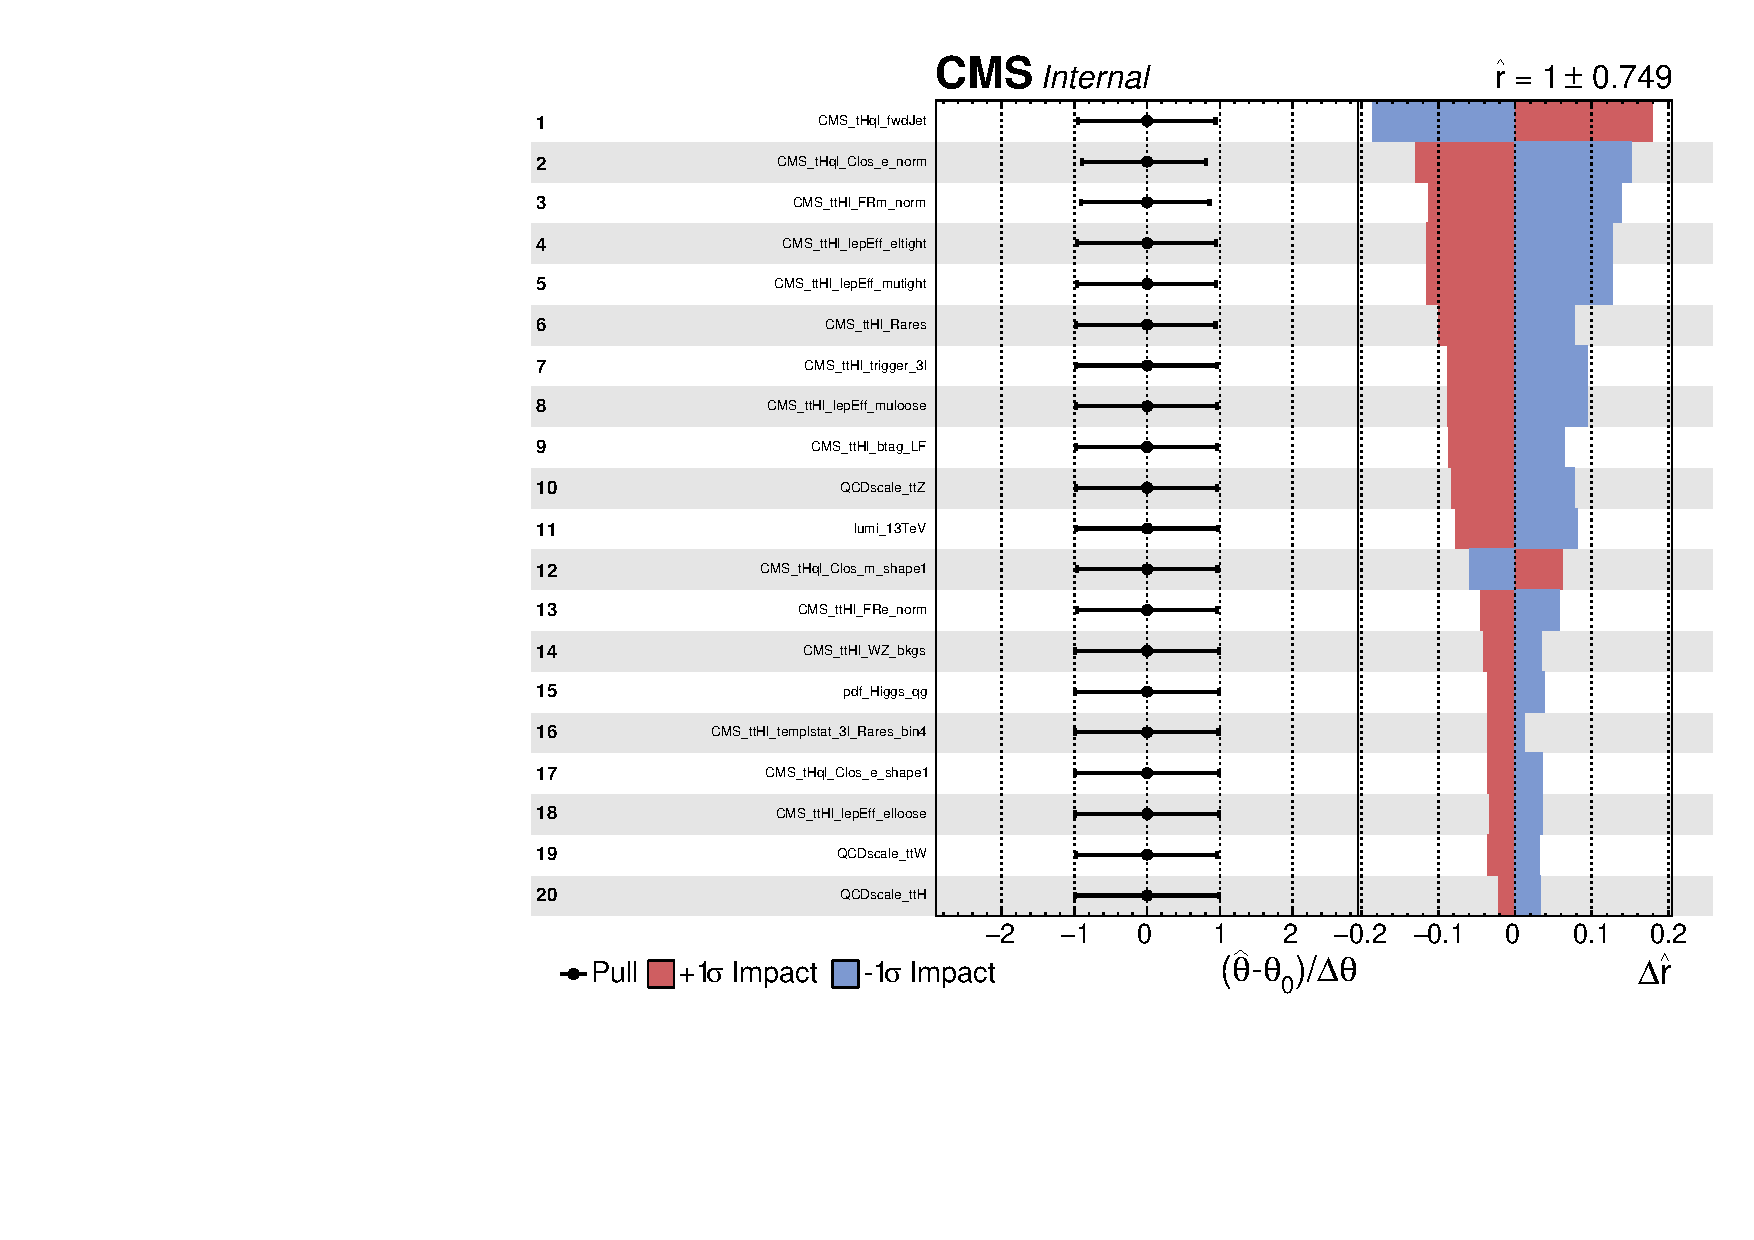
\includegraphics[width=1.0\textwidth]{limits/impacts/impacts_25.pdf}\\
\caption[Post-fit pulls and impacts with $\pt$ cut $25$ GeV for the forward jet]{Post-fit pulls and impacts of the 20 nuisance parameters with $\pt$ cut of $25$ GeV for the forward jet.}
\label{fig:impact25}
\end{figure}

\begin{figure} [!h]
 \centering
 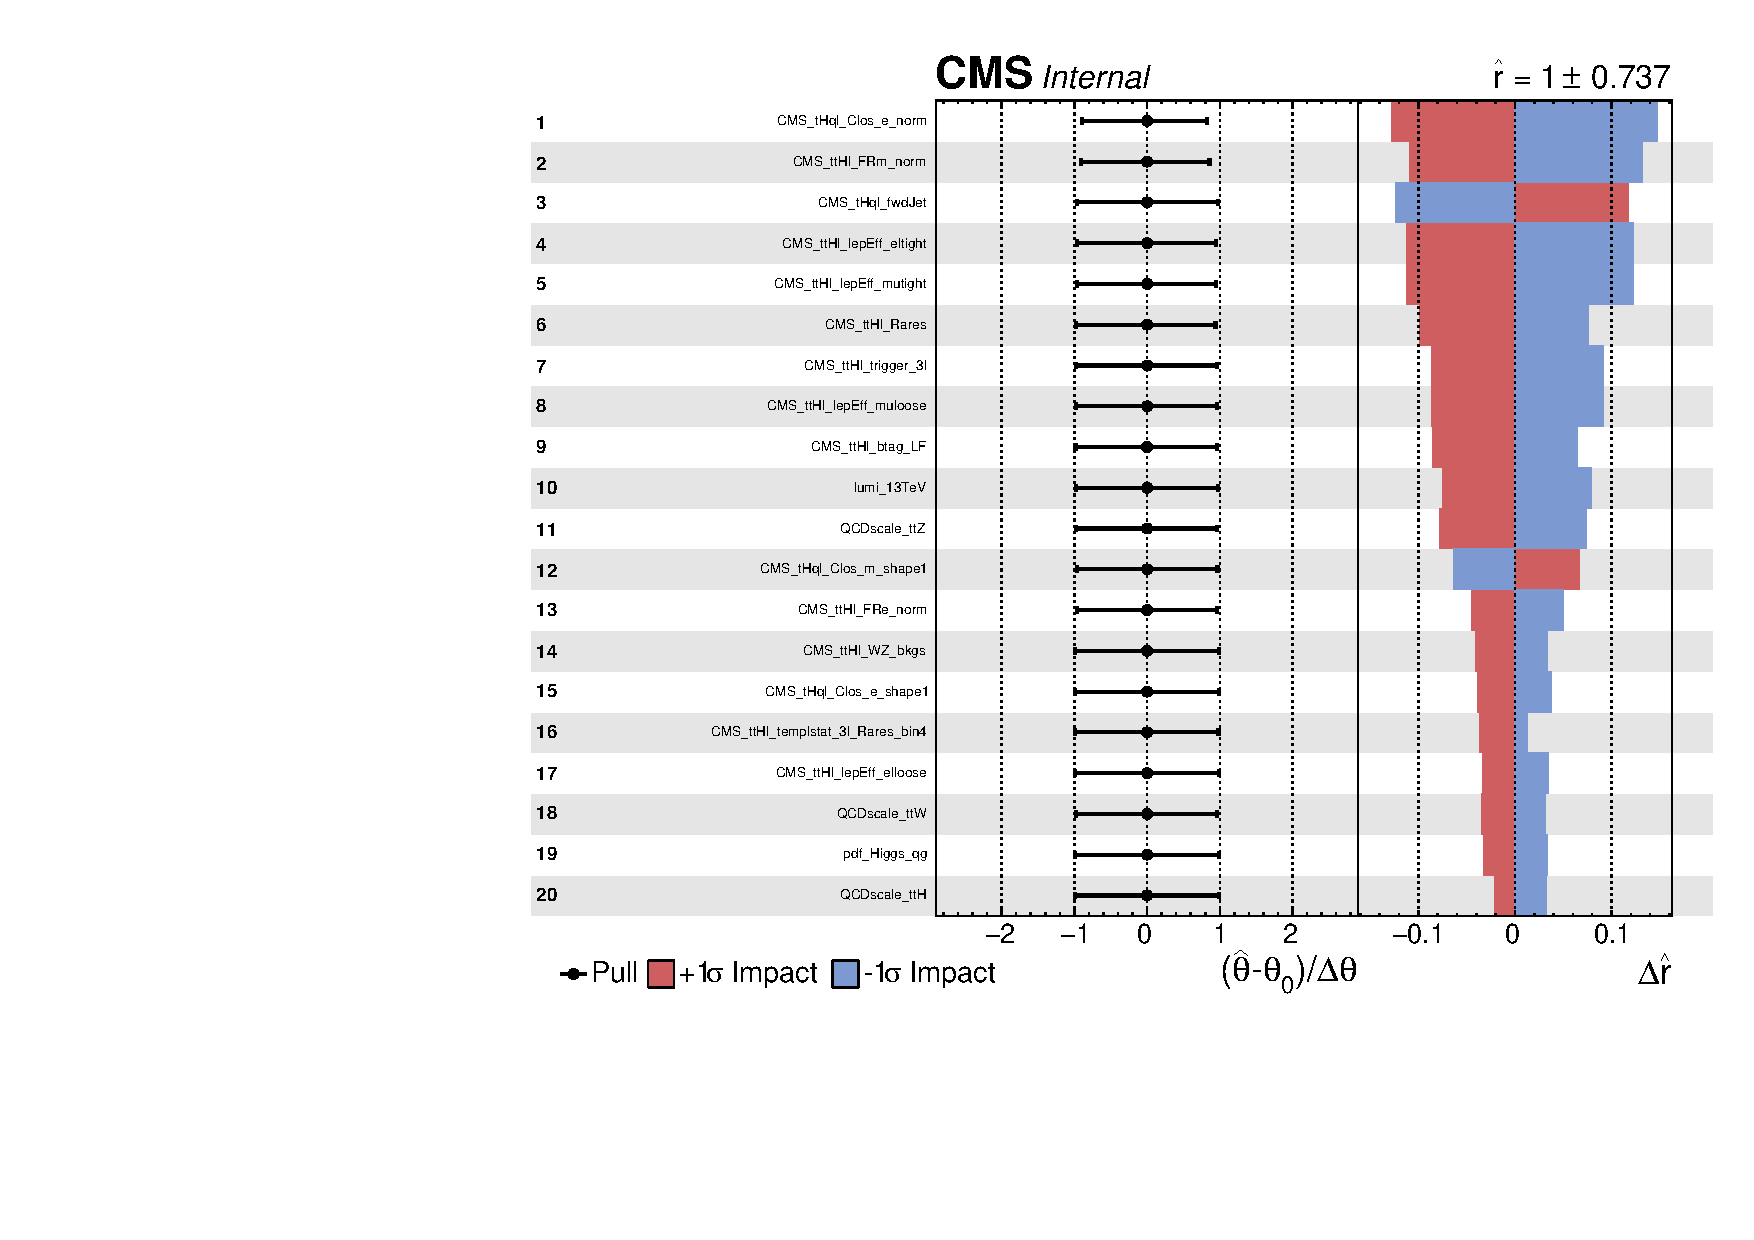
\includegraphics[width=1.0\textwidth]{limits/impacts/impacts_30.pdf}\\
\caption[Post-fit pulls and impacts with $\pt$ cut $30$ GeV for the forward jet]{Post-fit pulls and impacts of the 20 nuisance parameters with $\pt$ cut of $30$ GeV for the forward jet.}
\label{fig:impact30}
\end{figure}

\begin{figure} [!h]
 \centering
 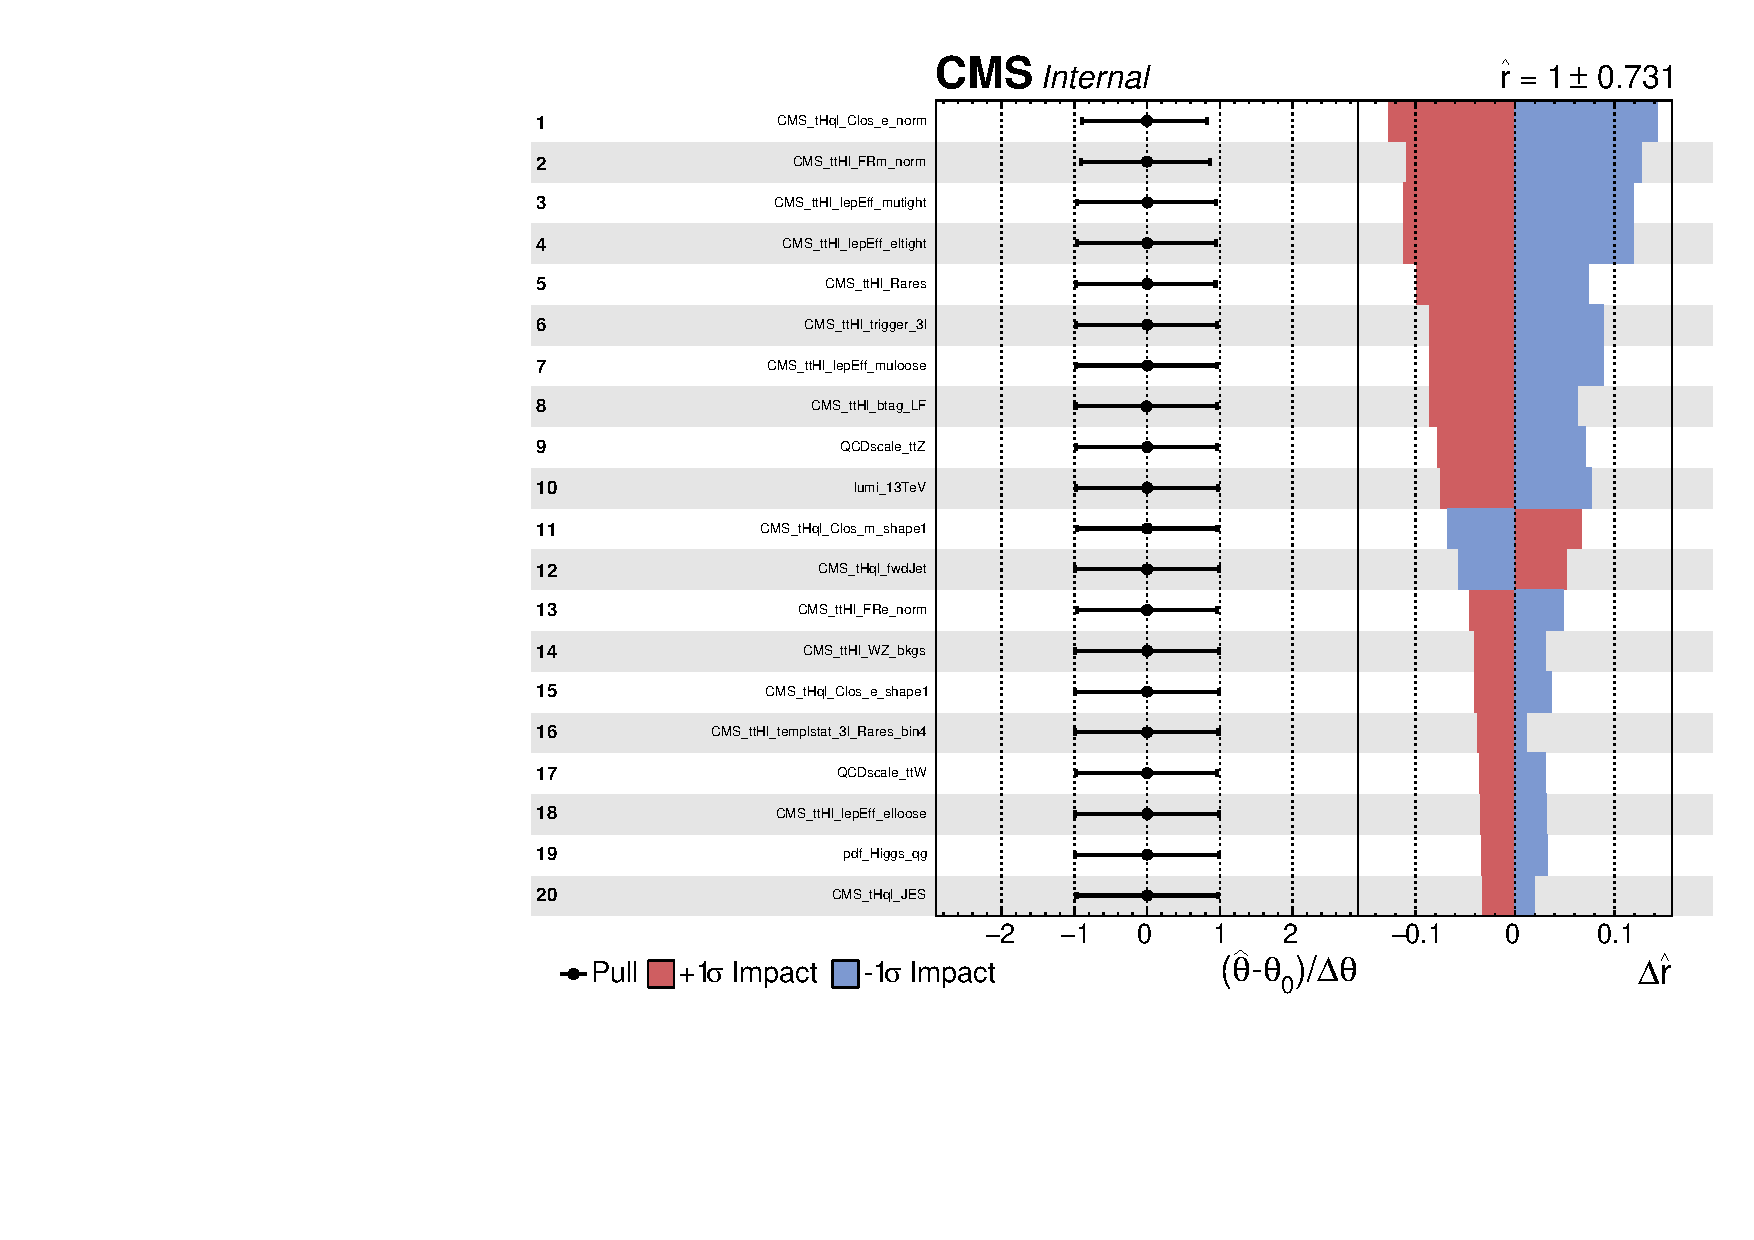
\includegraphics[width=1.0\textwidth]{limits/impacts/impacts_40.pdf}\\
\caption[Post-fit pulls and impacts with $\pt$ cut $25$ GeV for the forward jet]{Post-fit pulls and impacts of the 20 nuisance parameters with $\pt$ cut of $40$ GeV for the forward jet.}
\label{fig:impact40}
\end{figure}
